\chapter{Heterogeneous Reaction}

We will now be extending the methodology we have built up over the
previous chapters to a more complicated electrochemical reaciton
invoving two redox reaction and a heterogeneous chemical reaction
that couples the product and the reactant from the two equations
which occurs at the surface of the working electrode.

\begin{equation}\label{eq:hetero}
  \begin{gathered}
    \mathrm{A}+\mathrm{e}^{-} \rightleftarrows \mathrm{B} \\
    \mathrm{~B} \xrightarrow{k_{\text {het }}} \mathrm{C} \\
    \mathrm{C}+\mathrm{e}^{-} \rightleftarrows \mathrm{D}
  \end{gathered}
\end{equation}

This type of reaction appears in electroreduction of
halonitroaromatic compounds in aprotic media \cite{compton2014understanding}.

%TODO: Mention something about a more detailed description of these
% systems needs the consideration of adsorption / desorption which we
% deal with in the next chapter

%TODO: Mention that we now have the charge coefficient, rate constant
% formal potential for both reactions and heterogeneous rate constant
% as parameters

\begin{figure}
  \centering
  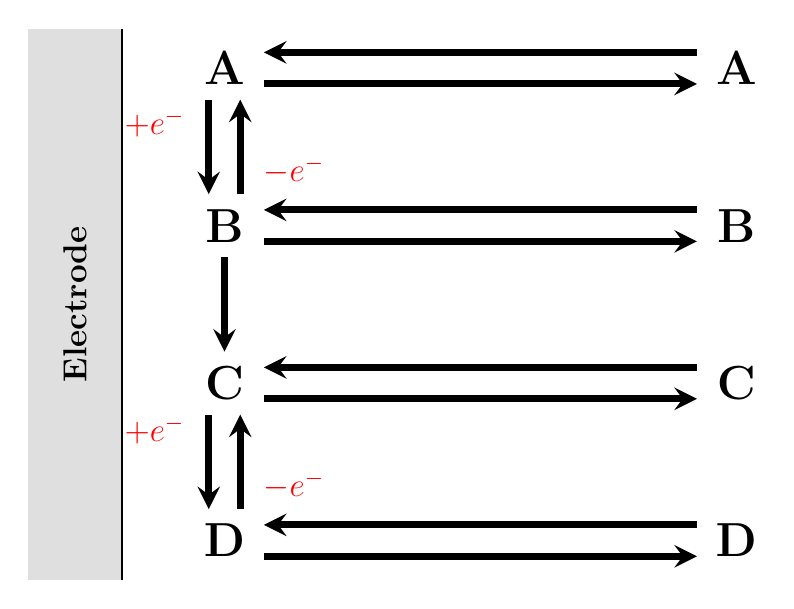
\begin{tikzpicture}[>=stealth, thick]
  % Electrode block
  \fill[gray!25] (-1.2, -1) rectangle (0, 6);
  \draw[thick] (0, -1) -- (0, 6);
  \node[rotate=90, font=\large\bfseries] at (-0.6, 2.5) {Electrode};
  % Species A row (top)
  \node[font=\LARGE\bfseries] at (1.3, 5.5) {A};
  \node[font=\LARGE\bfseries] at (7.8, 5.5) {A};
  % A: arrow from bulk towards electrode
  \draw[->, line width=2.5pt] (7.3, 5.7) -- (1.8, 5.7);
  % A: arrow from electrode towards bulk
  \draw[->, line width=2.5pt] (1.8, 5.3) -- (7.3, 5.3);
  % Species B row (bottom)
  \node[font=\LARGE\bfseries] at (1.3, 3.5) {B};
  \node[font=\LARGE\bfseries] at (7.8, 3.5) {B};
  % B: arrow from bulk towards electrode
  \draw[->, line width=2.5pt] (7.3, 3.7) -- (1.8, 3.7);
  % B: arrow from electrode towards bulk
  \draw[->, line width=2.5pt] (1.8, 3.3) -- (7.3, 3.3);
  % Electron transfer arrows AB
  \draw[->, line width=2.5pt] (1.1, 5.1) -- (1.1, 3.9);
  \node[right, font=\large] at (-0.1, 4.8) {\textcolor{red}{$+e^-$}};
  \draw[->, line width=2.5pt] (1.5, 3.9) -- (1.5, 5.1);
  \node[left, font=\large] at (2.7, 4.2) {\textcolor{red}{$-e^-$}};
  % Chemical Reaction B -> C
  \draw[->, line width=2.5pt] (1.3, 3.1) -- (1.3, 1.9);
  \node[font=\LARGE\bfseries] at (1.3, 1.5) {C};
  \node[font=\LARGE\bfseries] at (7.8, 1.5) {C};
  % C: arrow from bulk towards electrode
  \draw[->, line width=2.5pt] (7.3, 1.7) -- (1.8, 1.7);
  % C: arrow from electrode towards bulk
  \draw[->, line width=2.5pt] (1.8, 1.3) -- (7.3, 1.3);
  \node[font=\LARGE\bfseries] at (1.3, -0.5) {D};
  \node[font=\LARGE\bfseries] at (7.8, -0.5) {D};
  % D: arrow from bulk towards electrode
  \draw[->, line width=2.5pt] (7.3, -0.3) -- (1.8, -0.3);
  % D: arrow from electrode towards bulk
  \draw[->, line width=2.5pt] (1.8, -0.7) -- (7.3, -0.7);
  % Electron transfer arrows CD
  \draw[->, line width=2.5pt] (1.1, 1.1) -- (1.1, -0.1);
  \node[right, font=\large] at (-0.1, 0.9) {\textcolor{red}{$+e^-$}};
  \draw[->, line width=2.5pt] (1.5, -0.1) -- (1.5, 1.1);
  \node[left, font=\large] at (2.7, 0.2) {\textcolor{red}{$-e^-$}};
\end{tikzpicture}

  \caption{}
\end{figure}

\section{Mathematical Description}
We are able to express the reaction using the same non-dimensional
scheme as for the electron reaction. Only that we now need to model
the A, B, C and D species in separate governing equations. The
electrode boundary conditions change to:
\begin{equation}
  \begin{aligned}
    D_{\mathrm{A}}\left(\frac{\partial c_{\mathrm{A}}}{\partial
    x}\right)_{x=0} & =k_{\text {red }}^{(1)} c_{\mathrm{A}}(0,
    t)-k_{\mathrm{ox}}^{(1)} c_{\mathrm{B}}(0, t) \\
    D_{\mathrm{B}}\left(\frac{\partial c_{\mathrm{B}}}{\partial
    x}\right)_{x=0} & =-k_{\text {red }}^{(1)} c_{\mathrm{A}}(0,
    t)+k_{\mathrm{ox}}^{(1)} c_{\mathrm{B}}(0, t)+k_{\text {het }}
    c_{\mathrm{B}}(0, t) \\
    D_{\mathrm{C}}\left(\frac{\partial c_{\mathrm{C}}}{\partial
    x}\right)_{x=0} & =k_{\text {red }}^{(2)} c_{\mathrm{C}}(0,
    t)-k_{\mathrm{ox}}^{(2)} c_{\mathrm{D}}(0, t)-k_{\text {het }}
    c_{\mathrm{B}}(0, t) \\
    D_{\mathrm{D}}\left(\frac{\partial c_{\mathrm{D}}}{\partial
    x}\right)_{x=0} & =-k_{\text {red }}^{(2)} c_{\mathrm{C}}(0,
    t)+k_{\mathrm{ox}}^{(2)} c_{\mathrm{D}}(0, t)
  \end{aligned}
\end{equation}

Using the non-dimensional as we have described before and assuming
equal diffusion coefficients:
\begin{equation}
  \begin{aligned}
    & T>0, X=0: \\
    & \quad\left(\frac{\partial C_{\mathrm{A}}}{\partial
    X}\right)_{X=0}=K_{\text {red }}^{(1)} C_{\mathrm{A}}(0,
    T)-K_{\text {ox }}^{(1)} C_{\mathrm{B}}(0, T) \\
    & \quad\left(\frac{\partial C_{\mathrm{B}}}{\partial
    X}\right)_{X=0}=-K_{\text {red
    }}^{(1)} C_{\mathrm{A}}(0, T)+\left(K_{\text {ox }}^{(1)}+K_{\text
    {het }}\right) C_{\mathrm{B}}(0, T)\\
    & \quad\left(\frac{\partial C_{\mathrm{C}}}{\partial
    X}\right)_{X=0}=K_{\text {red
    }}^{(2)} C_{\mathrm{C}}(0, T)-K_{\text {ox }}^{(2)}
    C_{\mathrm{D}}(0, T)-K_{\text {het }} C_{\mathrm{B}}(0, T) \\
    & \quad\left(\frac{\partial C_{\mathrm{D}}}{\partial
    X}\right)_{X=0}=-K_{\text {red
    }}^{(2)} C_{\mathrm{C}}(0, T)+K_{\text {ox }}^{(2)}
    C_{\mathrm{D}}(0, T)
  \end{aligned}
\end{equation}
where the dimensionless rate constant of the heterogeneous chemical
reaction is given by
\begin{equation}
  K_{\mathrm{het}}=\frac{k_{\mathrm{het}} \epsilon}{D_{\mathrm{A}}}
\end{equation}

Notice the $K_{\mathrm{het}}$ term in the boundary for both
$\mathrm{B}$ and $\mathrm{C}$.
Regarding the current response the
total current will be given by the sum of the contribution of the
different heterogeneous \emph{electrochemical} reactions:
\begin{equation}
  \frac{I}{\mathrm{~F} A}
  =-\left\{D_{\mathrm{A}}\left(\frac{\partial
      c_{\mathrm{A}}}{\partial
    x}\right)_{x=0}+D_{\mathrm{C}}\left(\frac{\partial
    c_{\mathrm{C}}}{\partial x}\right)_{x=0}+k_{\text {het }}
  c_{\mathrm{B}}(0, t)\right\} \\
\end{equation}

% TODO: Mention the dimensionless conditions as everything is zero except A.
